% Created by tikzDevice version 0.6.2-92-0ad2792 on 2013-04-07 23:57:40
% !TEX encoding = UTF-8 Unicode
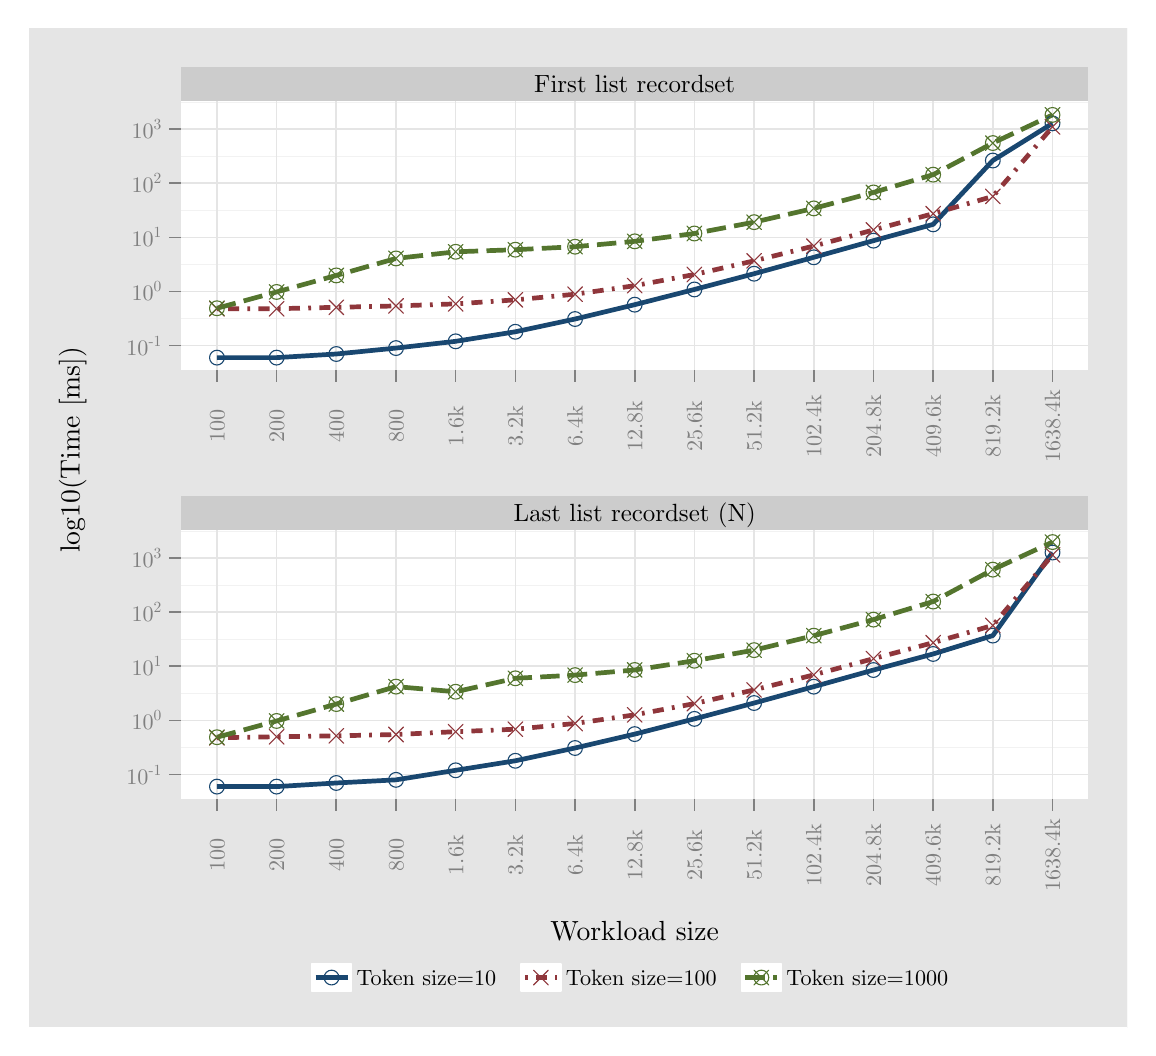
\begin{tikzpicture}[x=1pt,y=1pt]
\definecolor[named]{fillColor}{rgb}{1.00,1.00,1.00}
\path[use as bounding box,fill=fillColor,fill opacity=0.00] (0,0) rectangle (397.48,361.35);
\begin{scope}
\path[clip] (  0.00,  0.00) rectangle (397.48,361.35);
\definecolor[named]{drawColor}{rgb}{1.00,1.00,1.00}
\definecolor[named]{fillColor}{rgb}{0.90,0.90,0.90}

\path[draw=drawColor,line width= 0.6pt,line join=round,line cap=round,fill=fillColor] (  0.00, -0.00) rectangle (397.48,361.35);
\end{scope}
\begin{scope}
\path[clip] ( 55.45,237.71) rectangle (383.26,334.90);
\definecolor[named]{fillColor}{rgb}{1.00,1.00,1.00}

\path[fill=fillColor] ( 55.45,237.71) rectangle (383.26,334.90);
\definecolor[named]{drawColor}{rgb}{0.95,0.95,0.95}

\path[draw=drawColor,line width= 0.3pt,line join=round] ( 55.45,256.24) --
	(383.26,256.24);

\path[draw=drawColor,line width= 0.3pt,line join=round] ( 55.45,275.80) --
	(383.26,275.80);

\path[draw=drawColor,line width= 0.3pt,line join=round] ( 55.45,295.36) --
	(383.26,295.36);

\path[draw=drawColor,line width= 0.3pt,line join=round] ( 55.45,314.92) --
	(383.26,314.92);

\path[draw=drawColor,line width= 0.3pt,line join=round] ( 55.45,334.48) --
	(383.26,334.48);
\definecolor[named]{drawColor}{rgb}{0.90,0.90,0.90}

\path[draw=drawColor,line width= 0.6pt,line join=round] ( 55.45,246.46) --
	(383.26,246.46);

\path[draw=drawColor,line width= 0.6pt,line join=round] ( 55.45,266.02) --
	(383.26,266.02);

\path[draw=drawColor,line width= 0.6pt,line join=round] ( 55.45,285.58) --
	(383.26,285.58);

\path[draw=drawColor,line width= 0.6pt,line join=round] ( 55.45,305.14) --
	(383.26,305.14);

\path[draw=drawColor,line width= 0.6pt,line join=round] ( 55.45,324.70) --
	(383.26,324.70);

\path[draw=drawColor,line width= 0.6pt,line join=round] ( 68.39,237.71) --
	( 68.39,334.90);

\path[draw=drawColor,line width= 0.6pt,line join=round] ( 89.95,237.71) --
	( 89.95,334.90);

\path[draw=drawColor,line width= 0.6pt,line join=round] (111.52,237.71) --
	(111.52,334.90);

\path[draw=drawColor,line width= 0.6pt,line join=round] (133.09,237.71) --
	(133.09,334.90);

\path[draw=drawColor,line width= 0.6pt,line join=round] (154.65,237.71) --
	(154.65,334.90);

\path[draw=drawColor,line width= 0.6pt,line join=round] (176.22,237.71) --
	(176.22,334.90);

\path[draw=drawColor,line width= 0.6pt,line join=round] (197.79,237.71) --
	(197.79,334.90);

\path[draw=drawColor,line width= 0.6pt,line join=round] (219.35,237.71) --
	(219.35,334.90);

\path[draw=drawColor,line width= 0.6pt,line join=round] (240.92,237.71) --
	(240.92,334.90);

\path[draw=drawColor,line width= 0.6pt,line join=round] (262.49,237.71) --
	(262.49,334.90);

\path[draw=drawColor,line width= 0.6pt,line join=round] (284.05,237.71) --
	(284.05,334.90);

\path[draw=drawColor,line width= 0.6pt,line join=round] (305.62,237.71) --
	(305.62,334.90);

\path[draw=drawColor,line width= 0.6pt,line join=round] (327.19,237.71) --
	(327.19,334.90);

\path[draw=drawColor,line width= 0.6pt,line join=round] (348.75,237.71) --
	(348.75,334.90);

\path[draw=drawColor,line width= 0.6pt,line join=round] (370.32,237.71) --
	(370.32,334.90);
\definecolor[named]{drawColor}{rgb}{0.10,0.28,0.44}

\path[draw=drawColor,line width= 1.7pt,line join=round] ( 68.39,242.12) --
	( 89.95,242.12) --
	(111.52,243.43) --
	(133.09,245.57) --
	(154.65,248.01) --
	(176.22,251.46) --
	(197.79,256.07) --
	(219.35,261.25) --
	(240.92,266.75) --
	(262.49,272.44) --
	(284.05,278.37) --
	(305.62,284.38) --
	(327.19,290.27) --
	(348.75,313.34) --
	(370.32,326.77);
\definecolor[named]{drawColor}{rgb}{0.56,0.21,0.23}

\path[draw=drawColor,line width= 1.7pt,dash pattern=on 1pt off 3pt on 4pt off 3pt ,line join=round] ( 68.39,259.79) --
	( 89.95,259.79) --
	(111.52,260.30) --
	(133.09,260.79) --
	(154.65,261.54) --
	(176.22,262.99) --
	(197.79,265.03) --
	(219.35,268.12) --
	(240.92,272.16) --
	(262.49,277.09) --
	(284.05,282.44) --
	(305.62,288.25) --
	(327.19,294.14) --
	(348.75,300.37) --
	(370.32,325.48);
\definecolor[named]{drawColor}{rgb}{0.33,0.46,0.18}

\path[draw=drawColor,line width= 1.7pt,dash pattern=on 7pt off 3pt ,line join=round] ( 68.39,259.96) --
	( 89.95,265.85) --
	(111.52,271.82) --
	(133.09,277.96) --
	(154.65,280.36) --
	(176.22,281.11) --
	(197.79,282.20) --
	(219.35,284.14) --
	(240.92,286.97) --
	(262.49,291.07) --
	(284.05,296.04) --
	(305.62,301.81) --
	(327.19,308.23) --
	(348.75,319.65) --
	(370.32,329.82);
\definecolor[named]{drawColor}{rgb}{0.10,0.28,0.44}

\path[draw=drawColor,line width= 0.4pt,line join=round,line cap=round] ( 68.39,242.12) circle (  2.67);

\path[draw=drawColor,line width= 0.4pt,line join=round,line cap=round] ( 89.95,242.12) circle (  2.67);

\path[draw=drawColor,line width= 0.4pt,line join=round,line cap=round] (111.52,243.43) circle (  2.67);

\path[draw=drawColor,line width= 0.4pt,line join=round,line cap=round] (133.09,245.57) circle (  2.67);

\path[draw=drawColor,line width= 0.4pt,line join=round,line cap=round] (154.65,248.01) circle (  2.67);

\path[draw=drawColor,line width= 0.4pt,line join=round,line cap=round] (176.22,251.46) circle (  2.67);

\path[draw=drawColor,line width= 0.4pt,line join=round,line cap=round] (197.79,256.07) circle (  2.67);

\path[draw=drawColor,line width= 0.4pt,line join=round,line cap=round] (219.35,261.25) circle (  2.67);

\path[draw=drawColor,line width= 0.4pt,line join=round,line cap=round] (240.92,266.75) circle (  2.67);

\path[draw=drawColor,line width= 0.4pt,line join=round,line cap=round] (262.49,272.44) circle (  2.67);

\path[draw=drawColor,line width= 0.4pt,line join=round,line cap=round] (284.05,278.37) circle (  2.67);

\path[draw=drawColor,line width= 0.4pt,line join=round,line cap=round] (305.62,284.38) circle (  2.67);

\path[draw=drawColor,line width= 0.4pt,line join=round,line cap=round] (327.19,290.27) circle (  2.67);

\path[draw=drawColor,line width= 0.4pt,line join=round,line cap=round] (348.75,313.34) circle (  2.67);

\path[draw=drawColor,line width= 0.4pt,line join=round,line cap=round] (370.32,326.77) circle (  2.67);
\definecolor[named]{drawColor}{rgb}{0.56,0.21,0.23}

\path[draw=drawColor,line width= 0.4pt,line join=round,line cap=round,fill=fillColor] ( 65.72,257.12) -- ( 71.06,262.45);

\path[draw=drawColor,line width= 0.4pt,line join=round,line cap=round,fill=fillColor] ( 65.72,262.45) -- ( 71.06,257.12);

\path[draw=drawColor,line width= 0.4pt,line join=round,line cap=round,fill=fillColor] ( 87.29,257.12) -- ( 92.62,262.45);

\path[draw=drawColor,line width= 0.4pt,line join=round,line cap=round,fill=fillColor] ( 87.29,262.45) -- ( 92.62,257.12);

\path[draw=drawColor,line width= 0.4pt,line join=round,line cap=round,fill=fillColor] (108.85,257.63) -- (114.19,262.97);

\path[draw=drawColor,line width= 0.4pt,line join=round,line cap=round,fill=fillColor] (108.85,262.97) -- (114.19,257.63);

\path[draw=drawColor,line width= 0.4pt,line join=round,line cap=round,fill=fillColor] (130.42,258.12) -- (135.76,263.45);

\path[draw=drawColor,line width= 0.4pt,line join=round,line cap=round,fill=fillColor] (130.42,263.45) -- (135.76,258.12);

\path[draw=drawColor,line width= 0.4pt,line join=round,line cap=round,fill=fillColor] (151.99,258.87) -- (157.32,264.21);

\path[draw=drawColor,line width= 0.4pt,line join=round,line cap=round,fill=fillColor] (151.99,264.21) -- (157.32,258.87);

\path[draw=drawColor,line width= 0.4pt,line join=round,line cap=round,fill=fillColor] (173.55,260.32) -- (178.89,265.66);

\path[draw=drawColor,line width= 0.4pt,line join=round,line cap=round,fill=fillColor] (173.55,265.66) -- (178.89,260.32);

\path[draw=drawColor,line width= 0.4pt,line join=round,line cap=round,fill=fillColor] (195.12,262.36) -- (200.45,267.70);

\path[draw=drawColor,line width= 0.4pt,line join=round,line cap=round,fill=fillColor] (195.12,267.70) -- (200.45,262.36);

\path[draw=drawColor,line width= 0.4pt,line join=round,line cap=round,fill=fillColor] (216.69,265.45) -- (222.02,270.79);

\path[draw=drawColor,line width= 0.4pt,line join=round,line cap=round,fill=fillColor] (216.69,270.79) -- (222.02,265.45);

\path[draw=drawColor,line width= 0.4pt,line join=round,line cap=round,fill=fillColor] (238.25,269.49) -- (243.59,274.83);

\path[draw=drawColor,line width= 0.4pt,line join=round,line cap=round,fill=fillColor] (238.25,274.83) -- (243.59,269.49);

\path[draw=drawColor,line width= 0.4pt,line join=round,line cap=round,fill=fillColor] (259.82,274.42) -- (265.15,279.76);

\path[draw=drawColor,line width= 0.4pt,line join=round,line cap=round,fill=fillColor] (259.82,279.76) -- (265.15,274.42);

\path[draw=drawColor,line width= 0.4pt,line join=round,line cap=round,fill=fillColor] (281.39,279.77) -- (286.72,285.11);

\path[draw=drawColor,line width= 0.4pt,line join=round,line cap=round,fill=fillColor] (281.39,285.11) -- (286.72,279.77);

\path[draw=drawColor,line width= 0.4pt,line join=round,line cap=round,fill=fillColor] (302.95,285.59) -- (308.29,290.92);

\path[draw=drawColor,line width= 0.4pt,line join=round,line cap=round,fill=fillColor] (302.95,290.92) -- (308.29,285.59);

\path[draw=drawColor,line width= 0.4pt,line join=round,line cap=round,fill=fillColor] (324.52,291.47) -- (329.85,296.81);

\path[draw=drawColor,line width= 0.4pt,line join=round,line cap=round,fill=fillColor] (324.52,296.81) -- (329.85,291.47);

\path[draw=drawColor,line width= 0.4pt,line join=round,line cap=round,fill=fillColor] (346.08,297.70) -- (351.42,303.03);

\path[draw=drawColor,line width= 0.4pt,line join=round,line cap=round,fill=fillColor] (346.08,303.03) -- (351.42,297.70);

\path[draw=drawColor,line width= 0.4pt,line join=round,line cap=round,fill=fillColor] (367.65,322.81) -- (372.99,328.15);

\path[draw=drawColor,line width= 0.4pt,line join=round,line cap=round,fill=fillColor] (367.65,328.15) -- (372.99,322.81);
\definecolor[named]{drawColor}{rgb}{0.33,0.46,0.18}

\path[draw=drawColor,line width= 0.4pt,line join=round,line cap=round] ( 68.39,259.96) circle (  2.67);

\path[draw=drawColor,line width= 0.4pt,line join=round,line cap=round] ( 65.72,257.29) -- ( 71.06,262.63);

\path[draw=drawColor,line width= 0.4pt,line join=round,line cap=round] ( 65.72,262.63) -- ( 71.06,257.29);

\path[draw=drawColor,line width= 0.4pt,line join=round,line cap=round] ( 89.95,265.85) circle (  2.67);

\path[draw=drawColor,line width= 0.4pt,line join=round,line cap=round] ( 87.29,263.18) -- ( 92.62,268.52);

\path[draw=drawColor,line width= 0.4pt,line join=round,line cap=round] ( 87.29,268.52) -- ( 92.62,263.18);

\path[draw=drawColor,line width= 0.4pt,line join=round,line cap=round] (111.52,271.82) circle (  2.67);

\path[draw=drawColor,line width= 0.4pt,line join=round,line cap=round] (108.85,269.16) -- (114.19,274.49);

\path[draw=drawColor,line width= 0.4pt,line join=round,line cap=round] (108.85,274.49) -- (114.19,269.16);

\path[draw=drawColor,line width= 0.4pt,line join=round,line cap=round] (133.09,277.96) circle (  2.67);

\path[draw=drawColor,line width= 0.4pt,line join=round,line cap=round] (130.42,275.30) -- (135.76,280.63);

\path[draw=drawColor,line width= 0.4pt,line join=round,line cap=round] (130.42,280.63) -- (135.76,275.30);

\path[draw=drawColor,line width= 0.4pt,line join=round,line cap=round] (154.65,280.36) circle (  2.67);

\path[draw=drawColor,line width= 0.4pt,line join=round,line cap=round] (151.99,277.69) -- (157.32,283.03);

\path[draw=drawColor,line width= 0.4pt,line join=round,line cap=round] (151.99,283.03) -- (157.32,277.69);

\path[draw=drawColor,line width= 0.4pt,line join=round,line cap=round] (176.22,281.11) circle (  2.67);

\path[draw=drawColor,line width= 0.4pt,line join=round,line cap=round] (173.55,278.44) -- (178.89,283.78);

\path[draw=drawColor,line width= 0.4pt,line join=round,line cap=round] (173.55,283.78) -- (178.89,278.44);

\path[draw=drawColor,line width= 0.4pt,line join=round,line cap=round] (197.79,282.20) circle (  2.67);

\path[draw=drawColor,line width= 0.4pt,line join=round,line cap=round] (195.12,279.54) -- (200.45,284.87);

\path[draw=drawColor,line width= 0.4pt,line join=round,line cap=round] (195.12,284.87) -- (200.45,279.54);

\path[draw=drawColor,line width= 0.4pt,line join=round,line cap=round] (219.35,284.14) circle (  2.67);

\path[draw=drawColor,line width= 0.4pt,line join=round,line cap=round] (216.69,281.47) -- (222.02,286.81);

\path[draw=drawColor,line width= 0.4pt,line join=round,line cap=round] (216.69,286.81) -- (222.02,281.47);

\path[draw=drawColor,line width= 0.4pt,line join=round,line cap=round] (240.92,286.97) circle (  2.67);

\path[draw=drawColor,line width= 0.4pt,line join=round,line cap=round] (238.25,284.30) -- (243.59,289.64);

\path[draw=drawColor,line width= 0.4pt,line join=round,line cap=round] (238.25,289.64) -- (243.59,284.30);

\path[draw=drawColor,line width= 0.4pt,line join=round,line cap=round] (262.49,291.07) circle (  2.67);

\path[draw=drawColor,line width= 0.4pt,line join=round,line cap=round] (259.82,288.40) -- (265.15,293.74);

\path[draw=drawColor,line width= 0.4pt,line join=round,line cap=round] (259.82,293.74) -- (265.15,288.40);

\path[draw=drawColor,line width= 0.4pt,line join=round,line cap=round] (284.05,296.04) circle (  2.67);

\path[draw=drawColor,line width= 0.4pt,line join=round,line cap=round] (281.39,293.37) -- (286.72,298.71);

\path[draw=drawColor,line width= 0.4pt,line join=round,line cap=round] (281.39,298.71) -- (286.72,293.37);

\path[draw=drawColor,line width= 0.4pt,line join=round,line cap=round] (305.62,301.81) circle (  2.67);

\path[draw=drawColor,line width= 0.4pt,line join=round,line cap=round] (302.95,299.14) -- (308.29,304.48);

\path[draw=drawColor,line width= 0.4pt,line join=round,line cap=round] (302.95,304.48) -- (308.29,299.14);

\path[draw=drawColor,line width= 0.4pt,line join=round,line cap=round] (327.19,308.23) circle (  2.67);

\path[draw=drawColor,line width= 0.4pt,line join=round,line cap=round] (324.52,305.56) -- (329.85,310.89);

\path[draw=drawColor,line width= 0.4pt,line join=round,line cap=round] (324.52,310.89) -- (329.85,305.56);

\path[draw=drawColor,line width= 0.4pt,line join=round,line cap=round] (348.75,319.65) circle (  2.67);

\path[draw=drawColor,line width= 0.4pt,line join=round,line cap=round] (346.08,316.99) -- (351.42,322.32);

\path[draw=drawColor,line width= 0.4pt,line join=round,line cap=round] (346.08,322.32) -- (351.42,316.99);

\path[draw=drawColor,line width= 0.4pt,line join=round,line cap=round] (370.32,329.82) circle (  2.67);

\path[draw=drawColor,line width= 0.4pt,line join=round,line cap=round] (367.65,327.15) -- (372.99,332.49);

\path[draw=drawColor,line width= 0.4pt,line join=round,line cap=round] (367.65,332.49) -- (372.99,327.15);
\end{scope}
\begin{scope}
\path[clip] ( 55.45, 82.69) rectangle (383.26,179.89);
\definecolor[named]{fillColor}{rgb}{1.00,1.00,1.00}

\path[fill=fillColor] ( 55.45, 82.69) rectangle (383.26,179.89);
\definecolor[named]{drawColor}{rgb}{0.95,0.95,0.95}

\path[draw=drawColor,line width= 0.3pt,line join=round] ( 55.45,101.23) --
	(383.26,101.23);

\path[draw=drawColor,line width= 0.3pt,line join=round] ( 55.45,120.79) --
	(383.26,120.79);

\path[draw=drawColor,line width= 0.3pt,line join=round] ( 55.45,140.34) --
	(383.26,140.34);

\path[draw=drawColor,line width= 0.3pt,line join=round] ( 55.45,159.90) --
	(383.26,159.90);

\path[draw=drawColor,line width= 0.3pt,line join=round] ( 55.45,179.46) --
	(383.26,179.46);
\definecolor[named]{drawColor}{rgb}{0.90,0.90,0.90}

\path[draw=drawColor,line width= 0.6pt,line join=round] ( 55.45, 91.45) --
	(383.26, 91.45);

\path[draw=drawColor,line width= 0.6pt,line join=round] ( 55.45,111.01) --
	(383.26,111.01);

\path[draw=drawColor,line width= 0.6pt,line join=round] ( 55.45,130.57) --
	(383.26,130.57);

\path[draw=drawColor,line width= 0.6pt,line join=round] ( 55.45,150.12) --
	(383.26,150.12);

\path[draw=drawColor,line width= 0.6pt,line join=round] ( 55.45,169.68) --
	(383.26,169.68);

\path[draw=drawColor,line width= 0.6pt,line join=round] ( 68.39, 82.69) --
	( 68.39,179.89);

\path[draw=drawColor,line width= 0.6pt,line join=round] ( 89.95, 82.69) --
	( 89.95,179.89);

\path[draw=drawColor,line width= 0.6pt,line join=round] (111.52, 82.69) --
	(111.52,179.89);

\path[draw=drawColor,line width= 0.6pt,line join=round] (133.09, 82.69) --
	(133.09,179.89);

\path[draw=drawColor,line width= 0.6pt,line join=round] (154.65, 82.69) --
	(154.65,179.89);

\path[draw=drawColor,line width= 0.6pt,line join=round] (176.22, 82.69) --
	(176.22,179.89);

\path[draw=drawColor,line width= 0.6pt,line join=round] (197.79, 82.69) --
	(197.79,179.89);

\path[draw=drawColor,line width= 0.6pt,line join=round] (219.35, 82.69) --
	(219.35,179.89);

\path[draw=drawColor,line width= 0.6pt,line join=round] (240.92, 82.69) --
	(240.92,179.89);

\path[draw=drawColor,line width= 0.6pt,line join=round] (262.49, 82.69) --
	(262.49,179.89);

\path[draw=drawColor,line width= 0.6pt,line join=round] (284.05, 82.69) --
	(284.05,179.89);

\path[draw=drawColor,line width= 0.6pt,line join=round] (305.62, 82.69) --
	(305.62,179.89);

\path[draw=drawColor,line width= 0.6pt,line join=round] (327.19, 82.69) --
	(327.19,179.89);

\path[draw=drawColor,line width= 0.6pt,line join=round] (348.75, 82.69) --
	(348.75,179.89);

\path[draw=drawColor,line width= 0.6pt,line join=round] (370.32, 82.69) --
	(370.32,179.89);
\definecolor[named]{drawColor}{rgb}{0.10,0.28,0.44}

\path[draw=drawColor,line width= 1.7pt,line join=round] ( 68.39, 87.11) --
	( 89.95, 87.11) --
	(111.52, 88.42) --
	(133.09, 89.55) --
	(154.65, 93.00) --
	(176.22, 96.44) --
	(197.79,101.06) --
	(219.35,106.08) --
	(240.92,111.58) --
	(262.49,117.31) --
	(284.05,123.22) --
	(305.62,129.23) --
	(327.19,135.04) --
	(348.75,141.68) --
	(370.32,171.69);
\definecolor[named]{drawColor}{rgb}{0.56,0.21,0.23}

\path[draw=drawColor,line width= 1.7pt,dash pattern=on 1pt off 3pt on 4pt off 3pt ,line join=round] ( 68.39,104.77) --
	( 89.95,105.12) --
	(111.52,105.45) --
	(133.09,105.93) --
	(154.65,106.95) --
	(176.22,107.85) --
	(197.79,109.92) --
	(219.35,113.04) --
	(240.92,117.10) --
	(262.49,122.05) --
	(284.05,127.49) --
	(305.62,133.34) --
	(327.19,139.12) --
	(348.75,145.35) --
	(370.32,170.84);
\definecolor[named]{drawColor}{rgb}{0.33,0.46,0.18}

\path[draw=drawColor,line width= 1.7pt,dash pattern=on 7pt off 3pt ,line join=round] ( 68.39,104.95) --
	( 89.95,110.83) --
	(111.52,116.94) --
	(133.09,123.24) --
	(154.65,121.38) --
	(176.22,126.24) --
	(197.79,127.40) --
	(219.35,129.25) --
	(240.92,132.59) --
	(262.49,136.42) --
	(284.05,141.64) --
	(305.62,147.45) --
	(327.19,153.98) --
	(348.75,165.51) --
	(370.32,175.47);
\definecolor[named]{drawColor}{rgb}{0.10,0.28,0.44}

\path[draw=drawColor,line width= 0.4pt,line join=round,line cap=round] ( 68.39, 87.11) circle (  2.67);

\path[draw=drawColor,line width= 0.4pt,line join=round,line cap=round] ( 89.95, 87.11) circle (  2.67);

\path[draw=drawColor,line width= 0.4pt,line join=round,line cap=round] (111.52, 88.42) circle (  2.67);

\path[draw=drawColor,line width= 0.4pt,line join=round,line cap=round] (133.09, 89.55) circle (  2.67);

\path[draw=drawColor,line width= 0.4pt,line join=round,line cap=round] (154.65, 93.00) circle (  2.67);

\path[draw=drawColor,line width= 0.4pt,line join=round,line cap=round] (176.22, 96.44) circle (  2.67);

\path[draw=drawColor,line width= 0.4pt,line join=round,line cap=round] (197.79,101.06) circle (  2.67);

\path[draw=drawColor,line width= 0.4pt,line join=round,line cap=round] (219.35,106.08) circle (  2.67);

\path[draw=drawColor,line width= 0.4pt,line join=round,line cap=round] (240.92,111.58) circle (  2.67);

\path[draw=drawColor,line width= 0.4pt,line join=round,line cap=round] (262.49,117.31) circle (  2.67);

\path[draw=drawColor,line width= 0.4pt,line join=round,line cap=round] (284.05,123.22) circle (  2.67);

\path[draw=drawColor,line width= 0.4pt,line join=round,line cap=round] (305.62,129.23) circle (  2.67);

\path[draw=drawColor,line width= 0.4pt,line join=round,line cap=round] (327.19,135.04) circle (  2.67);

\path[draw=drawColor,line width= 0.4pt,line join=round,line cap=round] (348.75,141.68) circle (  2.67);

\path[draw=drawColor,line width= 0.4pt,line join=round,line cap=round] (370.32,171.69) circle (  2.67);
\definecolor[named]{drawColor}{rgb}{0.56,0.21,0.23}

\path[draw=drawColor,line width= 0.4pt,line join=round,line cap=round,fill=fillColor] ( 65.72,102.10) -- ( 71.06,107.44);

\path[draw=drawColor,line width= 0.4pt,line join=round,line cap=round,fill=fillColor] ( 65.72,107.44) -- ( 71.06,102.10);

\path[draw=drawColor,line width= 0.4pt,line join=round,line cap=round,fill=fillColor] ( 87.29,102.45) -- ( 92.62,107.79);

\path[draw=drawColor,line width= 0.4pt,line join=round,line cap=round,fill=fillColor] ( 87.29,107.79) -- ( 92.62,102.45);

\path[draw=drawColor,line width= 0.4pt,line join=round,line cap=round,fill=fillColor] (108.85,102.78) -- (114.19,108.12);

\path[draw=drawColor,line width= 0.4pt,line join=round,line cap=round,fill=fillColor] (108.85,108.12) -- (114.19,102.78);

\path[draw=drawColor,line width= 0.4pt,line join=round,line cap=round,fill=fillColor] (130.42,103.26) -- (135.76,108.60);

\path[draw=drawColor,line width= 0.4pt,line join=round,line cap=round,fill=fillColor] (130.42,108.60) -- (135.76,103.26);

\path[draw=drawColor,line width= 0.4pt,line join=round,line cap=round,fill=fillColor] (151.99,104.28) -- (157.32,109.61);

\path[draw=drawColor,line width= 0.4pt,line join=round,line cap=round,fill=fillColor] (151.99,109.61) -- (157.32,104.28);

\path[draw=drawColor,line width= 0.4pt,line join=round,line cap=round,fill=fillColor] (173.55,105.19) -- (178.89,110.52);

\path[draw=drawColor,line width= 0.4pt,line join=round,line cap=round,fill=fillColor] (173.55,110.52) -- (178.89,105.19);

\path[draw=drawColor,line width= 0.4pt,line join=round,line cap=round,fill=fillColor] (195.12,107.25) -- (200.45,112.59);

\path[draw=drawColor,line width= 0.4pt,line join=round,line cap=round,fill=fillColor] (195.12,112.59) -- (200.45,107.25);

\path[draw=drawColor,line width= 0.4pt,line join=round,line cap=round,fill=fillColor] (216.69,110.37) -- (222.02,115.70);

\path[draw=drawColor,line width= 0.4pt,line join=round,line cap=round,fill=fillColor] (216.69,115.70) -- (222.02,110.37);

\path[draw=drawColor,line width= 0.4pt,line join=round,line cap=round,fill=fillColor] (238.25,114.44) -- (243.59,119.77);

\path[draw=drawColor,line width= 0.4pt,line join=round,line cap=round,fill=fillColor] (238.25,119.77) -- (243.59,114.44);

\path[draw=drawColor,line width= 0.4pt,line join=round,line cap=round,fill=fillColor] (259.82,119.38) -- (265.15,124.72);

\path[draw=drawColor,line width= 0.4pt,line join=round,line cap=round,fill=fillColor] (259.82,124.72) -- (265.15,119.38);

\path[draw=drawColor,line width= 0.4pt,line join=round,line cap=round,fill=fillColor] (281.39,124.82) -- (286.72,130.15);

\path[draw=drawColor,line width= 0.4pt,line join=round,line cap=round,fill=fillColor] (281.39,130.15) -- (286.72,124.82);

\path[draw=drawColor,line width= 0.4pt,line join=round,line cap=round,fill=fillColor] (302.95,130.67) -- (308.29,136.01);

\path[draw=drawColor,line width= 0.4pt,line join=round,line cap=round,fill=fillColor] (302.95,136.01) -- (308.29,130.67);

\path[draw=drawColor,line width= 0.4pt,line join=round,line cap=round,fill=fillColor] (324.52,136.45) -- (329.85,141.79);

\path[draw=drawColor,line width= 0.4pt,line join=round,line cap=round,fill=fillColor] (324.52,141.79) -- (329.85,136.45);

\path[draw=drawColor,line width= 0.4pt,line join=round,line cap=round,fill=fillColor] (346.08,142.68) -- (351.42,148.02);

\path[draw=drawColor,line width= 0.4pt,line join=round,line cap=round,fill=fillColor] (346.08,148.02) -- (351.42,142.68);

\path[draw=drawColor,line width= 0.4pt,line join=round,line cap=round,fill=fillColor] (367.65,168.17) -- (372.99,173.50);

\path[draw=drawColor,line width= 0.4pt,line join=round,line cap=round,fill=fillColor] (367.65,173.50) -- (372.99,168.17);
\definecolor[named]{drawColor}{rgb}{0.33,0.46,0.18}

\path[draw=drawColor,line width= 0.4pt,line join=round,line cap=round] ( 68.39,104.95) circle (  2.67);

\path[draw=drawColor,line width= 0.4pt,line join=round,line cap=round] ( 65.72,102.28) -- ( 71.06,107.61);

\path[draw=drawColor,line width= 0.4pt,line join=round,line cap=round] ( 65.72,107.61) -- ( 71.06,102.28);

\path[draw=drawColor,line width= 0.4pt,line join=round,line cap=round] ( 89.95,110.83) circle (  2.67);

\path[draw=drawColor,line width= 0.4pt,line join=round,line cap=round] ( 87.29,108.17) -- ( 92.62,113.50);

\path[draw=drawColor,line width= 0.4pt,line join=round,line cap=round] ( 87.29,113.50) -- ( 92.62,108.17);

\path[draw=drawColor,line width= 0.4pt,line join=round,line cap=round] (111.52,116.94) circle (  2.67);

\path[draw=drawColor,line width= 0.4pt,line join=round,line cap=round] (108.85,114.27) -- (114.19,119.60);

\path[draw=drawColor,line width= 0.4pt,line join=round,line cap=round] (108.85,119.60) -- (114.19,114.27);

\path[draw=drawColor,line width= 0.4pt,line join=round,line cap=round] (133.09,123.24) circle (  2.67);

\path[draw=drawColor,line width= 0.4pt,line join=round,line cap=round] (130.42,120.57) -- (135.76,125.90);

\path[draw=drawColor,line width= 0.4pt,line join=round,line cap=round] (130.42,125.90) -- (135.76,120.57);

\path[draw=drawColor,line width= 0.4pt,line join=round,line cap=round] (154.65,121.38) circle (  2.67);

\path[draw=drawColor,line width= 0.4pt,line join=round,line cap=round] (151.99,118.71) -- (157.32,124.04);

\path[draw=drawColor,line width= 0.4pt,line join=round,line cap=round] (151.99,124.04) -- (157.32,118.71);

\path[draw=drawColor,line width= 0.4pt,line join=round,line cap=round] (176.22,126.24) circle (  2.67);

\path[draw=drawColor,line width= 0.4pt,line join=round,line cap=round] (173.55,123.57) -- (178.89,128.91);

\path[draw=drawColor,line width= 0.4pt,line join=round,line cap=round] (173.55,128.91) -- (178.89,123.57);

\path[draw=drawColor,line width= 0.4pt,line join=round,line cap=round] (197.79,127.40) circle (  2.67);

\path[draw=drawColor,line width= 0.4pt,line join=round,line cap=round] (195.12,124.73) -- (200.45,130.07);

\path[draw=drawColor,line width= 0.4pt,line join=round,line cap=round] (195.12,130.07) -- (200.45,124.73);

\path[draw=drawColor,line width= 0.4pt,line join=round,line cap=round] (219.35,129.25) circle (  2.67);

\path[draw=drawColor,line width= 0.4pt,line join=round,line cap=round] (216.69,126.59) -- (222.02,131.92);

\path[draw=drawColor,line width= 0.4pt,line join=round,line cap=round] (216.69,131.92) -- (222.02,126.59);

\path[draw=drawColor,line width= 0.4pt,line join=round,line cap=round] (240.92,132.59) circle (  2.67);

\path[draw=drawColor,line width= 0.4pt,line join=round,line cap=round] (238.25,129.92) -- (243.59,135.26);

\path[draw=drawColor,line width= 0.4pt,line join=round,line cap=round] (238.25,135.26) -- (243.59,129.92);

\path[draw=drawColor,line width= 0.4pt,line join=round,line cap=round] (262.49,136.42) circle (  2.67);

\path[draw=drawColor,line width= 0.4pt,line join=round,line cap=round] (259.82,133.75) -- (265.15,139.09);

\path[draw=drawColor,line width= 0.4pt,line join=round,line cap=round] (259.82,139.09) -- (265.15,133.75);

\path[draw=drawColor,line width= 0.4pt,line join=round,line cap=round] (284.05,141.64) circle (  2.67);

\path[draw=drawColor,line width= 0.4pt,line join=round,line cap=round] (281.39,138.98) -- (286.72,144.31);

\path[draw=drawColor,line width= 0.4pt,line join=round,line cap=round] (281.39,144.31) -- (286.72,138.98);

\path[draw=drawColor,line width= 0.4pt,line join=round,line cap=round] (305.62,147.45) circle (  2.67);

\path[draw=drawColor,line width= 0.4pt,line join=round,line cap=round] (302.95,144.79) -- (308.29,150.12);

\path[draw=drawColor,line width= 0.4pt,line join=round,line cap=round] (302.95,150.12) -- (308.29,144.79);

\path[draw=drawColor,line width= 0.4pt,line join=round,line cap=round] (327.19,153.98) circle (  2.67);

\path[draw=drawColor,line width= 0.4pt,line join=round,line cap=round] (324.52,151.31) -- (329.85,156.65);

\path[draw=drawColor,line width= 0.4pt,line join=round,line cap=round] (324.52,156.65) -- (329.85,151.31);

\path[draw=drawColor,line width= 0.4pt,line join=round,line cap=round] (348.75,165.51) circle (  2.67);

\path[draw=drawColor,line width= 0.4pt,line join=round,line cap=round] (346.08,162.84) -- (351.42,168.18);

\path[draw=drawColor,line width= 0.4pt,line join=round,line cap=round] (346.08,168.18) -- (351.42,162.84);

\path[draw=drawColor,line width= 0.4pt,line join=round,line cap=round] (370.32,175.47) circle (  2.67);

\path[draw=drawColor,line width= 0.4pt,line join=round,line cap=round] (367.65,172.80) -- (372.99,178.14);

\path[draw=drawColor,line width= 0.4pt,line join=round,line cap=round] (367.65,178.14) -- (372.99,172.80);
\end{scope}
\begin{scope}
\path[clip] (  0.00,  0.00) rectangle (397.48,361.35);
\definecolor[named]{fillColor}{rgb}{0.80,0.80,0.80}

\path[fill=fillColor] ( 55.45,334.90) rectangle (383.26,347.12);
\definecolor[named]{drawColor}{rgb}{0.00,0.00,0.00}

\node[text=drawColor,anchor=base,inner sep=0pt, outer sep=0pt, scale=  0.90] at (219.35,337.91) {First list recordset };
\end{scope}
\begin{scope}
\path[clip] (  0.00,  0.00) rectangle (397.48,361.35);
\definecolor[named]{fillColor}{rgb}{0.80,0.80,0.80}

\path[fill=fillColor] ( 55.45,179.89) rectangle (383.26,192.11);
\definecolor[named]{drawColor}{rgb}{0.00,0.00,0.00}

\node[text=drawColor,anchor=base,inner sep=0pt, outer sep=0pt, scale=  0.90] at (219.35,182.90) {Last list recordset (N) };
\end{scope}
\begin{scope}
\path[clip] (  0.00,  0.00) rectangle (397.48,361.35);
\definecolor[named]{drawColor}{rgb}{0.50,0.50,0.50}

\node[text=drawColor,anchor=base west,inner sep=0pt, outer sep=0pt, scale=  0.80] at ( 35.67,243.03) {10};

\node[text=drawColor,anchor=base west,inner sep=0pt, outer sep=0pt, scale=  0.56] at ( 43.67,246.30) {-};

\node[text=drawColor,anchor=base west,inner sep=0pt, outer sep=0pt, scale=  0.56] at ( 45.54,246.30) {1};

\node[text=drawColor,anchor=base west,inner sep=0pt, outer sep=0pt, scale=  0.80] at ( 37.54,262.59) {10};

\node[text=drawColor,anchor=base west,inner sep=0pt, outer sep=0pt, scale=  0.56] at ( 45.54,265.86) {0};

\node[text=drawColor,anchor=base west,inner sep=0pt, outer sep=0pt, scale=  0.80] at ( 37.54,282.15) {10};

\node[text=drawColor,anchor=base west,inner sep=0pt, outer sep=0pt, scale=  0.56] at ( 45.54,285.42) {1};

\node[text=drawColor,anchor=base west,inner sep=0pt, outer sep=0pt, scale=  0.80] at ( 37.54,301.71) {10};

\node[text=drawColor,anchor=base west,inner sep=0pt, outer sep=0pt, scale=  0.56] at ( 45.54,304.98) {2};

\node[text=drawColor,anchor=base west,inner sep=0pt, outer sep=0pt, scale=  0.80] at ( 37.54,321.27) {10};

\node[text=drawColor,anchor=base west,inner sep=0pt, outer sep=0pt, scale=  0.56] at ( 45.54,324.54) {3};
\end{scope}
\begin{scope}
\path[clip] (  0.00,  0.00) rectangle (397.48,361.35);
\definecolor[named]{drawColor}{rgb}{0.50,0.50,0.50}

\path[draw=drawColor,line width= 0.6pt,line join=round] ( 51.18,246.46) --
	( 55.45,246.46);

\path[draw=drawColor,line width= 0.6pt,line join=round] ( 51.18,266.02) --
	( 55.45,266.02);

\path[draw=drawColor,line width= 0.6pt,line join=round] ( 51.18,285.58) --
	( 55.45,285.58);

\path[draw=drawColor,line width= 0.6pt,line join=round] ( 51.18,305.14) --
	( 55.45,305.14);

\path[draw=drawColor,line width= 0.6pt,line join=round] ( 51.18,324.70) --
	( 55.45,324.70);
\end{scope}
\begin{scope}
\path[clip] (  0.00,  0.00) rectangle (397.48,361.35);
\definecolor[named]{drawColor}{rgb}{0.50,0.50,0.50}

\node[text=drawColor,anchor=base west,inner sep=0pt, outer sep=0pt, scale=  0.80] at ( 35.67, 88.02) {10};

\node[text=drawColor,anchor=base west,inner sep=0pt, outer sep=0pt, scale=  0.56] at ( 43.67, 91.29) {-};

\node[text=drawColor,anchor=base west,inner sep=0pt, outer sep=0pt, scale=  0.56] at ( 45.54, 91.29) {1};

\node[text=drawColor,anchor=base west,inner sep=0pt, outer sep=0pt, scale=  0.80] at ( 37.54,107.57) {10};

\node[text=drawColor,anchor=base west,inner sep=0pt, outer sep=0pt, scale=  0.56] at ( 45.54,110.85) {0};

\node[text=drawColor,anchor=base west,inner sep=0pt, outer sep=0pt, scale=  0.80] at ( 37.54,127.13) {10};

\node[text=drawColor,anchor=base west,inner sep=0pt, outer sep=0pt, scale=  0.56] at ( 45.54,130.40) {1};

\node[text=drawColor,anchor=base west,inner sep=0pt, outer sep=0pt, scale=  0.80] at ( 37.54,146.69) {10};

\node[text=drawColor,anchor=base west,inner sep=0pt, outer sep=0pt, scale=  0.56] at ( 45.54,149.96) {2};

\node[text=drawColor,anchor=base west,inner sep=0pt, outer sep=0pt, scale=  0.80] at ( 37.54,166.25) {10};

\node[text=drawColor,anchor=base west,inner sep=0pt, outer sep=0pt, scale=  0.56] at ( 45.54,169.52) {3};
\end{scope}
\begin{scope}
\path[clip] (  0.00,  0.00) rectangle (397.48,361.35);
\definecolor[named]{drawColor}{rgb}{0.50,0.50,0.50}

\path[draw=drawColor,line width= 0.6pt,line join=round] ( 51.18, 91.45) --
	( 55.45, 91.45);

\path[draw=drawColor,line width= 0.6pt,line join=round] ( 51.18,111.01) --
	( 55.45,111.01);

\path[draw=drawColor,line width= 0.6pt,line join=round] ( 51.18,130.57) --
	( 55.45,130.57);

\path[draw=drawColor,line width= 0.6pt,line join=round] ( 51.18,150.12) --
	( 55.45,150.12);

\path[draw=drawColor,line width= 0.6pt,line join=round] ( 51.18,169.68) --
	( 55.45,169.68);
\end{scope}
\begin{scope}
\path[clip] (  0.00,  0.00) rectangle (397.48,361.35);
\definecolor[named]{drawColor}{rgb}{0.50,0.50,0.50}

\path[draw=drawColor,line width= 0.6pt,line join=round] ( 68.39,233.44) --
	( 68.39,237.71);

\path[draw=drawColor,line width= 0.6pt,line join=round] ( 89.95,233.44) --
	( 89.95,237.71);

\path[draw=drawColor,line width= 0.6pt,line join=round] (111.52,233.44) --
	(111.52,237.71);

\path[draw=drawColor,line width= 0.6pt,line join=round] (133.09,233.44) --
	(133.09,237.71);

\path[draw=drawColor,line width= 0.6pt,line join=round] (154.65,233.44) --
	(154.65,237.71);

\path[draw=drawColor,line width= 0.6pt,line join=round] (176.22,233.44) --
	(176.22,237.71);

\path[draw=drawColor,line width= 0.6pt,line join=round] (197.79,233.44) --
	(197.79,237.71);

\path[draw=drawColor,line width= 0.6pt,line join=round] (219.35,233.44) --
	(219.35,237.71);

\path[draw=drawColor,line width= 0.6pt,line join=round] (240.92,233.44) --
	(240.92,237.71);

\path[draw=drawColor,line width= 0.6pt,line join=round] (262.49,233.44) --
	(262.49,237.71);

\path[draw=drawColor,line width= 0.6pt,line join=round] (284.05,233.44) --
	(284.05,237.71);

\path[draw=drawColor,line width= 0.6pt,line join=round] (305.62,233.44) --
	(305.62,237.71);

\path[draw=drawColor,line width= 0.6pt,line join=round] (327.19,233.44) --
	(327.19,237.71);

\path[draw=drawColor,line width= 0.6pt,line join=round] (348.75,233.44) --
	(348.75,237.71);

\path[draw=drawColor,line width= 0.6pt,line join=round] (370.32,233.44) --
	(370.32,237.71);
\end{scope}
\begin{scope}
\path[clip] (  0.00,  0.00) rectangle (397.48,361.35);
\definecolor[named]{drawColor}{rgb}{0.50,0.50,0.50}

\node[text=drawColor,rotate= 90.00,anchor=base,inner sep=0pt, outer sep=0pt, scale=  0.80] at ( 71.14,217.37) {100};

\node[text=drawColor,rotate= 90.00,anchor=base,inner sep=0pt, outer sep=0pt, scale=  0.80] at ( 92.71,217.37) {200};

\node[text=drawColor,rotate= 90.00,anchor=base,inner sep=0pt, outer sep=0pt, scale=  0.80] at (114.28,217.37) {400};

\node[text=drawColor,rotate= 90.00,anchor=base,inner sep=0pt, outer sep=0pt, scale=  0.80] at (135.84,217.37) {800};

\node[text=drawColor,rotate= 90.00,anchor=base,inner sep=0pt, outer sep=0pt, scale=  0.80] at (157.41,217.37) {1.6k};

\node[text=drawColor,rotate= 90.00,anchor=base,inner sep=0pt, outer sep=0pt, scale=  0.80] at (178.98,217.37) {3.2k};

\node[text=drawColor,rotate= 90.00,anchor=base,inner sep=0pt, outer sep=0pt, scale=  0.80] at (200.54,217.37) {6.4k};

\node[text=drawColor,rotate= 90.00,anchor=base,inner sep=0pt, outer sep=0pt, scale=  0.80] at (222.11,217.37) {12.8k};

\node[text=drawColor,rotate= 90.00,anchor=base,inner sep=0pt, outer sep=0pt, scale=  0.80] at (243.67,217.37) {25.6k};

\node[text=drawColor,rotate= 90.00,anchor=base,inner sep=0pt, outer sep=0pt, scale=  0.80] at (265.24,217.37) {51.2k};

\node[text=drawColor,rotate= 90.00,anchor=base,inner sep=0pt, outer sep=0pt, scale=  0.80] at (286.81,217.37) {102.4k};

\node[text=drawColor,rotate= 90.00,anchor=base,inner sep=0pt, outer sep=0pt, scale=  0.80] at (308.37,217.37) {204.8k};

\node[text=drawColor,rotate= 90.00,anchor=base,inner sep=0pt, outer sep=0pt, scale=  0.80] at (329.94,217.37) {409.6k};

\node[text=drawColor,rotate= 90.00,anchor=base,inner sep=0pt, outer sep=0pt, scale=  0.80] at (351.51,217.37) {819.2k};

\node[text=drawColor,rotate= 90.00,anchor=base,inner sep=0pt, outer sep=0pt, scale=  0.80] at (373.07,217.37) {1638.4k};
\end{scope}
\begin{scope}
\path[clip] (  0.00,  0.00) rectangle (397.48,361.35);
\definecolor[named]{drawColor}{rgb}{0.50,0.50,0.50}

\path[draw=drawColor,line width= 0.6pt,line join=round] ( 68.39, 78.42) --
	( 68.39, 82.69);

\path[draw=drawColor,line width= 0.6pt,line join=round] ( 89.95, 78.42) --
	( 89.95, 82.69);

\path[draw=drawColor,line width= 0.6pt,line join=round] (111.52, 78.42) --
	(111.52, 82.69);

\path[draw=drawColor,line width= 0.6pt,line join=round] (133.09, 78.42) --
	(133.09, 82.69);

\path[draw=drawColor,line width= 0.6pt,line join=round] (154.65, 78.42) --
	(154.65, 82.69);

\path[draw=drawColor,line width= 0.6pt,line join=round] (176.22, 78.42) --
	(176.22, 82.69);

\path[draw=drawColor,line width= 0.6pt,line join=round] (197.79, 78.42) --
	(197.79, 82.69);

\path[draw=drawColor,line width= 0.6pt,line join=round] (219.35, 78.42) --
	(219.35, 82.69);

\path[draw=drawColor,line width= 0.6pt,line join=round] (240.92, 78.42) --
	(240.92, 82.69);

\path[draw=drawColor,line width= 0.6pt,line join=round] (262.49, 78.42) --
	(262.49, 82.69);

\path[draw=drawColor,line width= 0.6pt,line join=round] (284.05, 78.42) --
	(284.05, 82.69);

\path[draw=drawColor,line width= 0.6pt,line join=round] (305.62, 78.42) --
	(305.62, 82.69);

\path[draw=drawColor,line width= 0.6pt,line join=round] (327.19, 78.42) --
	(327.19, 82.69);

\path[draw=drawColor,line width= 0.6pt,line join=round] (348.75, 78.42) --
	(348.75, 82.69);

\path[draw=drawColor,line width= 0.6pt,line join=round] (370.32, 78.42) --
	(370.32, 82.69);
\end{scope}
\begin{scope}
\path[clip] (  0.00,  0.00) rectangle (397.48,361.35);
\definecolor[named]{drawColor}{rgb}{0.50,0.50,0.50}

\node[text=drawColor,rotate= 90.00,anchor=base,inner sep=0pt, outer sep=0pt, scale=  0.80] at ( 71.14, 62.36) {100};

\node[text=drawColor,rotate= 90.00,anchor=base,inner sep=0pt, outer sep=0pt, scale=  0.80] at ( 92.71, 62.36) {200};

\node[text=drawColor,rotate= 90.00,anchor=base,inner sep=0pt, outer sep=0pt, scale=  0.80] at (114.28, 62.36) {400};

\node[text=drawColor,rotate= 90.00,anchor=base,inner sep=0pt, outer sep=0pt, scale=  0.80] at (135.84, 62.36) {800};

\node[text=drawColor,rotate= 90.00,anchor=base,inner sep=0pt, outer sep=0pt, scale=  0.80] at (157.41, 62.36) {1.6k};

\node[text=drawColor,rotate= 90.00,anchor=base,inner sep=0pt, outer sep=0pt, scale=  0.80] at (178.98, 62.36) {3.2k};

\node[text=drawColor,rotate= 90.00,anchor=base,inner sep=0pt, outer sep=0pt, scale=  0.80] at (200.54, 62.36) {6.4k};

\node[text=drawColor,rotate= 90.00,anchor=base,inner sep=0pt, outer sep=0pt, scale=  0.80] at (222.11, 62.36) {12.8k};

\node[text=drawColor,rotate= 90.00,anchor=base,inner sep=0pt, outer sep=0pt, scale=  0.80] at (243.67, 62.36) {25.6k};

\node[text=drawColor,rotate= 90.00,anchor=base,inner sep=0pt, outer sep=0pt, scale=  0.80] at (265.24, 62.36) {51.2k};

\node[text=drawColor,rotate= 90.00,anchor=base,inner sep=0pt, outer sep=0pt, scale=  0.80] at (286.81, 62.36) {102.4k};

\node[text=drawColor,rotate= 90.00,anchor=base,inner sep=0pt, outer sep=0pt, scale=  0.80] at (308.37, 62.36) {204.8k};

\node[text=drawColor,rotate= 90.00,anchor=base,inner sep=0pt, outer sep=0pt, scale=  0.80] at (329.94, 62.36) {409.6k};

\node[text=drawColor,rotate= 90.00,anchor=base,inner sep=0pt, outer sep=0pt, scale=  0.80] at (351.51, 62.36) {819.2k};

\node[text=drawColor,rotate= 90.00,anchor=base,inner sep=0pt, outer sep=0pt, scale=  0.80] at (373.07, 62.36) {1638.4k};
\end{scope}
\begin{scope}
\path[clip] (  0.00,  0.00) rectangle (397.48,361.35);
\definecolor[named]{drawColor}{rgb}{0.00,0.00,0.00}

\node[text=drawColor,anchor=base,inner sep=0pt, outer sep=0pt, scale=  1.00] at (219.35, 31.41) {Workload size};
\end{scope}
\begin{scope}
\path[clip] (  0.00,  0.00) rectangle (397.48,361.35);
\definecolor[named]{drawColor}{rgb}{0.00,0.00,0.00}

\node[text=drawColor,rotate= 90.00,anchor=base,inner sep=0pt, outer sep=0pt, scale=  1.00] at ( 18.80,208.80) {log10(Time [ms])};
\end{scope}
\begin{scope}
\path[clip] (  0.00,  0.00) rectangle (397.48,361.35);
\definecolor[named]{fillColor}{rgb}{0.90,0.90,0.90}

\path[fill=fillColor] ( 94.70,  8.87) rectangle (344.01, 27.36);
\end{scope}
\begin{scope}
\path[clip] (  0.00,  0.00) rectangle (397.48,361.35);
\definecolor[named]{drawColor}{rgb}{1.00,1.00,1.00}
\definecolor[named]{fillColor}{rgb}{1.00,1.00,1.00}

\path[draw=drawColor,line width= 0.6pt,line join=round,line cap=round,fill=fillColor] (102.58, 13.14) rectangle (117.04, 23.09);
\end{scope}
\begin{scope}
\path[clip] (  0.00,  0.00) rectangle (397.48,361.35);
\definecolor[named]{drawColor}{rgb}{0.10,0.28,0.44}

\path[draw=drawColor,line width= 1.7pt,line join=round] (104.03, 18.11) -- (115.59, 18.11);
\end{scope}
\begin{scope}
\path[clip] (  0.00,  0.00) rectangle (397.48,361.35);
\definecolor[named]{drawColor}{rgb}{0.10,0.28,0.44}

\path[draw=drawColor,line width= 0.4pt,line join=round,line cap=round] (109.81, 18.11) circle (  2.67);
\end{scope}
\begin{scope}
\path[clip] (  0.00,  0.00) rectangle (397.48,361.35);
\definecolor[named]{drawColor}{rgb}{1.00,1.00,1.00}
\definecolor[named]{fillColor}{rgb}{1.00,1.00,1.00}

\path[draw=drawColor,line width= 0.6pt,line join=round,line cap=round,fill=fillColor] (178.24, 13.14) rectangle (192.69, 23.09);
\end{scope}
\begin{scope}
\path[clip] (  0.00,  0.00) rectangle (397.48,361.35);
\definecolor[named]{drawColor}{rgb}{0.56,0.21,0.23}

\path[draw=drawColor,line width= 1.7pt,dash pattern=on 1pt off 3pt on 4pt off 3pt ,line join=round] (179.68, 18.11) -- (191.25, 18.11);
\end{scope}
\begin{scope}
\path[clip] (  0.00,  0.00) rectangle (397.48,361.35);
\definecolor[named]{drawColor}{rgb}{0.56,0.21,0.23}
\definecolor[named]{fillColor}{rgb}{1.00,1.00,1.00}

\path[draw=drawColor,line width= 0.4pt,line join=round,line cap=round,fill=fillColor] (182.80, 15.45) -- (188.13, 20.78);

\path[draw=drawColor,line width= 0.4pt,line join=round,line cap=round,fill=fillColor] (182.80, 20.78) -- (188.13, 15.45);
\end{scope}
\begin{scope}
\path[clip] (  0.00,  0.00) rectangle (397.48,361.35);
\definecolor[named]{drawColor}{rgb}{1.00,1.00,1.00}
\definecolor[named]{fillColor}{rgb}{1.00,1.00,1.00}

\path[draw=drawColor,line width= 0.6pt,line join=round,line cap=round,fill=fillColor] (257.89, 13.14) rectangle (272.35, 23.09);
\end{scope}
\begin{scope}
\path[clip] (  0.00,  0.00) rectangle (397.48,361.35);
\definecolor[named]{drawColor}{rgb}{0.33,0.46,0.18}

\path[draw=drawColor,line width= 1.7pt,dash pattern=on 7pt off 3pt ,line join=round] (259.34, 18.11) -- (270.90, 18.11);
\end{scope}
\begin{scope}
\path[clip] (  0.00,  0.00) rectangle (397.48,361.35);
\definecolor[named]{drawColor}{rgb}{0.33,0.46,0.18}

\path[draw=drawColor,line width= 0.4pt,line join=round,line cap=round] (265.12, 18.11) circle (  2.67);

\path[draw=drawColor,line width= 0.4pt,line join=round,line cap=round] (262.45, 15.45) -- (267.79, 20.78);

\path[draw=drawColor,line width= 0.4pt,line join=round,line cap=round] (262.45, 20.78) -- (267.79, 15.45);
\end{scope}
\begin{scope}
\path[clip] (  0.00,  0.00) rectangle (397.48,361.35);
\definecolor[named]{drawColor}{rgb}{0.00,0.00,0.00}

\node[text=drawColor,anchor=base west,inner sep=0pt, outer sep=0pt, scale=  0.80] at (118.84, 15.36) {Token size=10 $\;\;$};
\end{scope}
\begin{scope}
\path[clip] (  0.00,  0.00) rectangle (397.48,361.35);
\definecolor[named]{drawColor}{rgb}{0.00,0.00,0.00}

\node[text=drawColor,anchor=base west,inner sep=0pt, outer sep=0pt, scale=  0.80] at (194.50, 15.36) {Token size=100 $\;\;$};
\end{scope}
\begin{scope}
\path[clip] (  0.00,  0.00) rectangle (397.48,361.35);
\definecolor[named]{drawColor}{rgb}{0.00,0.00,0.00}

\node[text=drawColor,anchor=base west,inner sep=0pt, outer sep=0pt, scale=  0.80] at (274.15, 15.36) {Token size=1000 $\;\;$};
\end{scope}
\end{tikzpicture}
